\subsection{Sprachkonzepte}
    \label{solutionDetails:dslConcepts}
    Die \gls{wccdl} spiegelt die Konzepte aus
    Kapitel \ref{section:conceptClassesFeaturesSelectors}
    durch Linguistic Abstractions wider.
    Die folgende Beschreibung orientiert sich an den
    Domänenkonzepten.
    
    \paragraph*{Klassen}
    Abbildung \ref{image:dslClasses} modelliert,
    wie das Konzept der Klassen in der \gls{wccdl} abgebildet wird.

    \begin{figure}[htb]
        \centering
        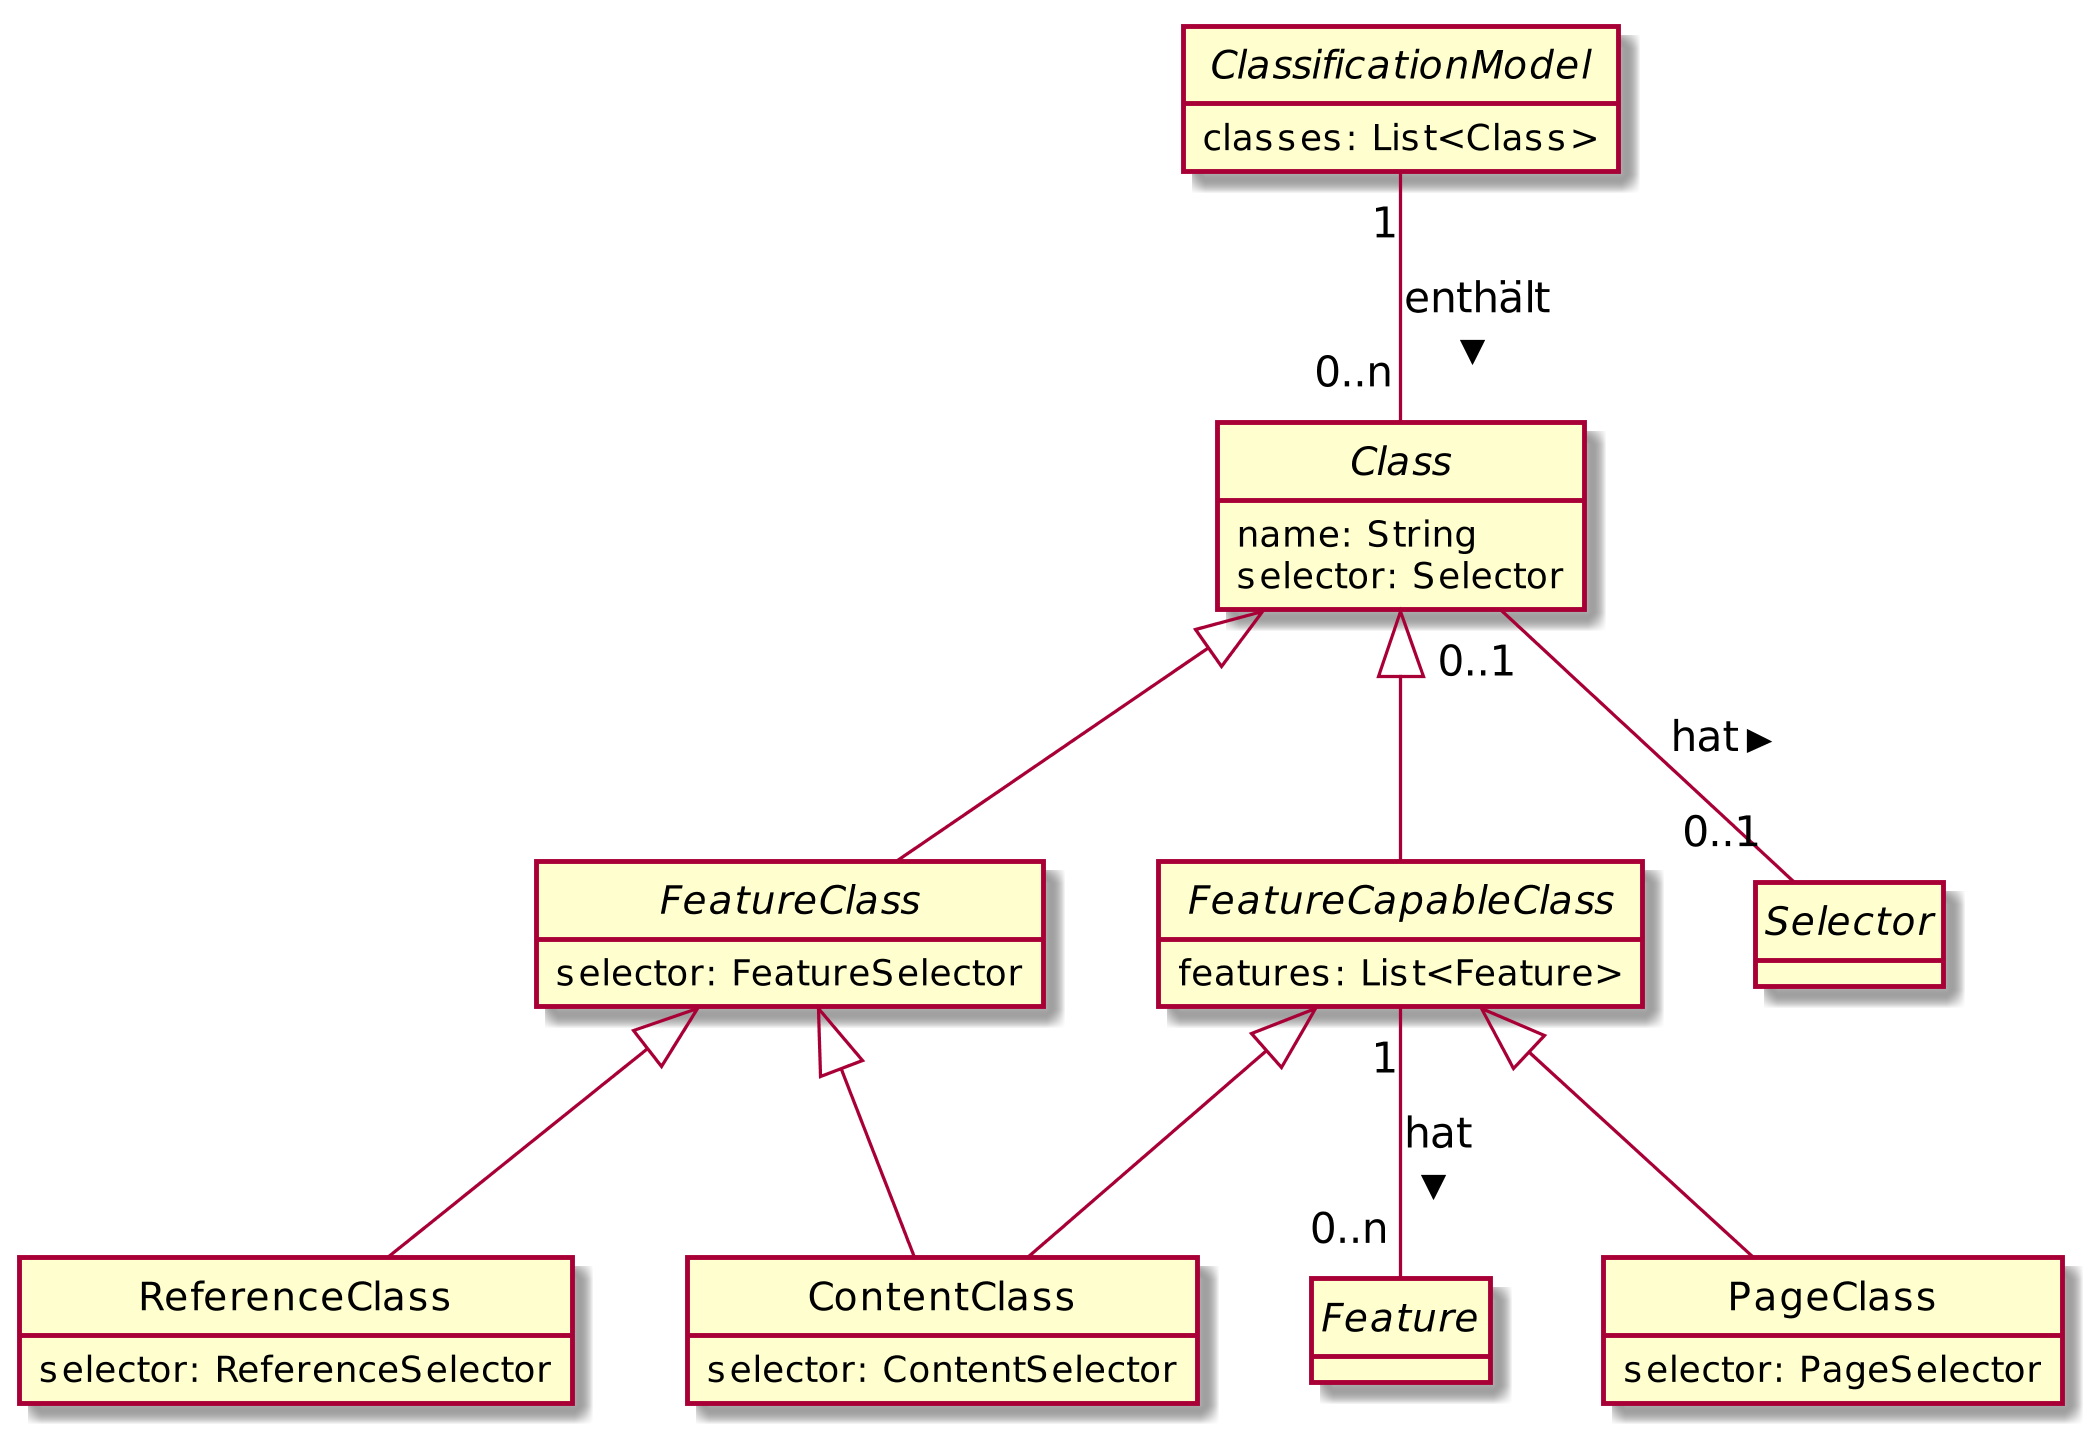
\includegraphics[scale=\imageScalingFactor]{../resources/dsl/classes.png}
        \caption{Klassen in der \acrshort{wccdl}}
        \label{image:dslClasses}
    \end{figure}

    Zentraler Bestandteil der Sprache ist das abstrakte Konzept \texttt{Class},
    welches gemäß der Domänenkonzepte in drei konkrete Ausprägungen unterteilt wird:
    \texttt{PageClass}, \texttt{ContentClass} und \texttt{ReferenceClass}.
    Jedes in der \gls{wccdl} geschriebene Programm ist eine Sammlung
    von Klassendefinitionen und enthält deshalb genau ein \texttt{ClassificationModel},
    das wiedrum beliebig viele Instanzen der genannten Konzepte beinhalten kann.
    Klassen besitzen einen Namen und einen Selektor,
    der -- ausgenommen von Seitenklassen -- optional ist.
    Die Sprache enthält hierzu das entsprechende Konzept \texttt{Selector},
    welches weiter unten vorgestellt wird.
    Da nicht jeder Selektor für jede Klasse geeignet ist,
    verwenden die einzelnen Klassentypen verschiedene Selektortypen,
    wobei es sich um \texttt{PageSelector}, \texttt{ContentSelector}
    und \texttt{ReferenceSelector} handelt,
    die ebenfalls später genauer thematisiert werden.
    Wieso der Selektor Teil der Typinformation von \texttt{ContentClass}
    und \texttt{ReferenceClass} ist,
    wird bei der unteren Diskussion der Features ersichtlich.
    Lediglich Seiten- und Inhaltsklassen können Features besitzen,
    weshalb die Sprache das Konzept \texttt{FeatureCapableClass} einführt,
    um diese Eigenschaft auszudrücken.
    \texttt{PageClass} und \texttt{ContentClass} sind
    Ableitungen dieses Konzeptes, welches
    wiederum eine Spezialisierung von \texttt{Class} ist.
    Auf der anderen Seite sind nur Inhalts- und Referenzklassen als Klasse eines Features geeignet.
    Für diese Eigenschaft enthält die Sprache das Konzept \texttt{FeatureClass},
    welches ebenfalls von \texttt{Class} erbt und
    von dem sowohl \texttt{ContentClass} als auch \texttt{ReferenceClass} ableiten.

    \paragraph*{Features}
    Die \gls{wccdl} repräsentiert Features über das gleichnamige Sprachkonzept,
    was Abbildung \ref{image:dslFeatures} veranschaulicht.
    Analog zum Domänenkonzept besitzt jedes Feature in der Sprache einen Namen
    und eine Klasse, welche vom oben vorgestellten Typ \texttt{FeatureClass} sein muss.
    Des Weiteren kann ein Feature einen Selektor besitzen,
    um den der Klasse für sich zu überschreiben.
    Da nicht jede Selektorart für Features geeignet ist,
    führt die Sprache das Konzept \texttt{FeatureSelector} ein,
    um eine Unterscheidung zwischen geeigneten und ungeeigneten Arten möglich zu machen.
    Auf \texttt{FeatureSelector} wird weiter unten genauer eingegangen.
    In Bezug auf den Selektor eines Features ist außerdem relevant,
    ob dieser für die Klasse des Features geeignet ist.
    Das heißt, ob der Selektor zum Beispiel ein \texttt{ContentSelector} ist,
    wenn es sich bei der Klasse um eine Inhaltsklasse handelt.
    Dies wird sichergestellt,
    indem der Typ des Selektors Teil der Typinformation von
    \texttt{Feature} ist und sowohl die Eigenschaften \texttt{class} als auch
    \texttt{selector} diesen verwenden und damit zueinanderpassen müssen.
    Ob es sich bei einem Feature um ein {\scalarFeature} oder ein {\collectionFeature} handelt,
    ist aus Sicht der Sprache lediglich eine boolesche Eigenschaft und erfordert
    keine weitere Unterscheidung.
    Das ist eine Abweichung vom Modell des Domänenkonzeptes, die dadurch begründet ist,
    dass die Sprache Features lediglich deklariert und nicht sicherstellen muss,
    dass in einer konkreten Klassifikation alle Elemente eines {\collectionFeature}s die gleiche Klasse verwenden.
    Eine Unterscheidung zwischen {\contentFeature}s und {\referenceFeature}s
    ist ebenfalls nicht notwendig,
    da diese Information klar aus der verwendeten \texttt{FeatureClass} hervorgeht.

    \begin{figure}[tb]
        \centering
        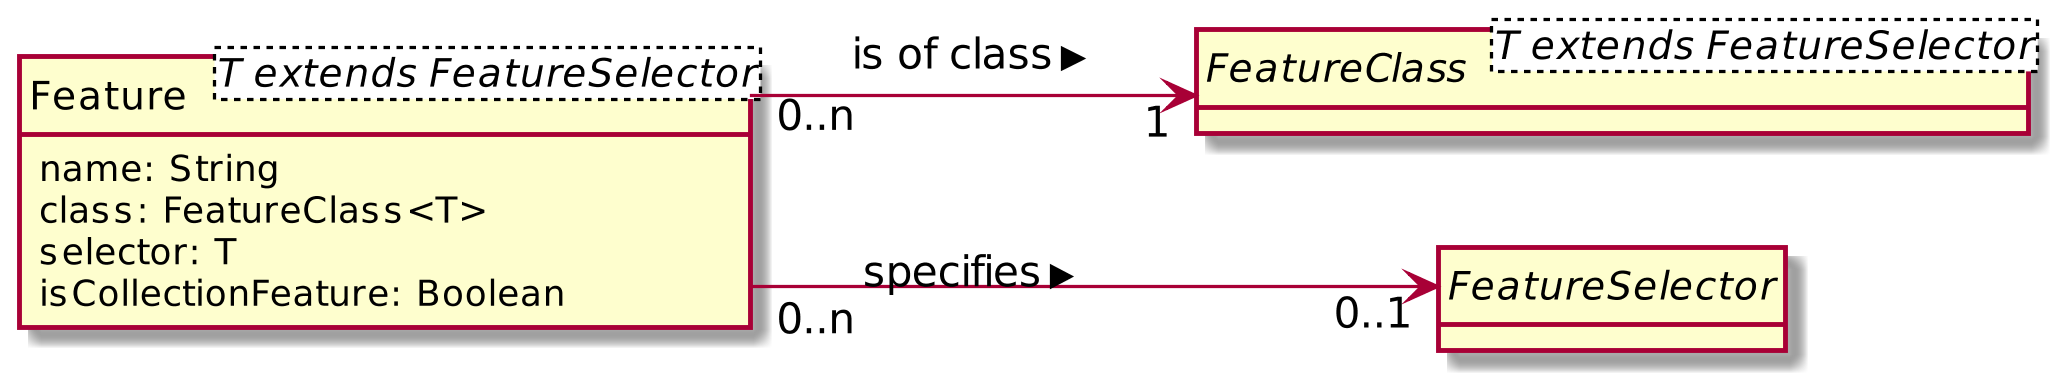
\includegraphics[scale=\imageScalingFactor]{../resources/dsl/features.png}
        \caption{Features in der \acrshort{wccdl}}
        \label{image:dslFeatures}
    \end{figure}

    \paragraph*{Selektoren}
    Die \gls{wccdl} bietet des Weiteren Konzepte zur Definition von Selektoren,
    die vereinzelt schon angesprochen wurden.
    Eine vollständige Übersicht bietet Abbildung \ref{image:dslSelectors}.

    \begin{figure}[htb]
        \centering
        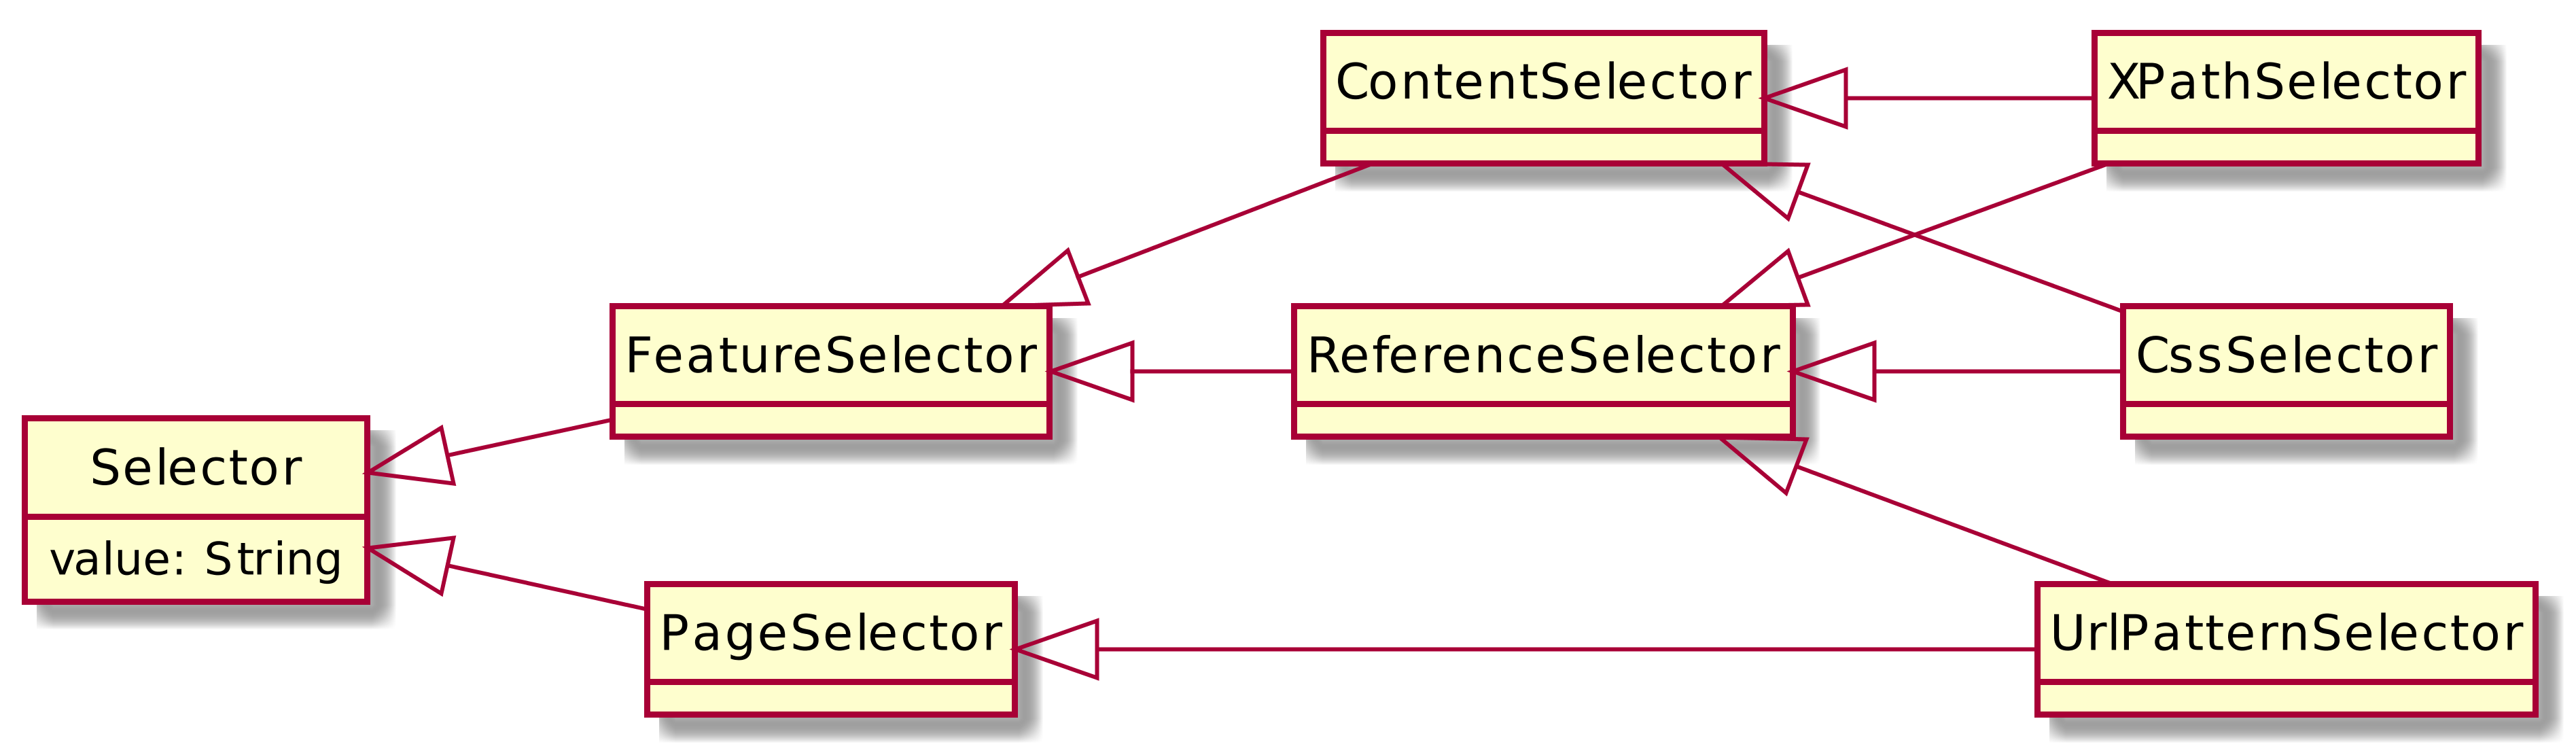
\includegraphics[scale=\imageScalingFactor]{../resources/dsl/selectors.png}
        \caption{Selektoren in der WCML}
        \label{image:dslSelectors}
    \end{figure}

    Das abstrakte Konzept \texttt{Selector} entspricht dem gleichnamigen Domänenkonzept
    und unterteilt sich in weitere abstrakte Konzepte,
    mit denen Selektoren nach ihrer Eignung für die verschiedenen Klassentypen getrennt werden.
    Diese Konzepte sind \texttt{PageSelector}, \texttt{ContentSelector} und \texttt{ReferenceSelector}.
    Die vom Klassifizierungssystem unterstützten
    Selektoren\footnote{vgl. Kapitel \ref{section:conceptSupportedSelectors}}
    spiegelt die \gls{wccdl} mit den konkreten Konzepten
    \texttt{CssSelector}, \texttt{XPathSelector} und \texttt{UrlPatternSelector} wider,
    die die zuvor genannten Konzepte spezialisieren.
    Dadurch wird eindeutig abgebildet, welche Selektorarten für welche Klassentypen geeignet sind.
    Ein weiterer relevanter Aspekt ist die Eignung der Selektoren für Features,
    wozu das bereits erwähnte Konzept \texttt{FeatureSelector} existiert.
    Da Features nur Inhalts- oder Referenzklassen verwenden können,
    leiten nur \texttt{ContentSelector} und \texttt{ReferenceSelector} von diesem ab.
    